\documentclass{standalone}

\usepackage{tikz}
\usepackage[T1]{fontenc}
\usepackage[tt=false, type1=true]{libertine}
\usepackage[varqu]{zi4}
\usepackage[libertine]{newtxmath}

\usetikzlibrary{shapes, positioning, calc}

\begin{document}

{\scriptsize
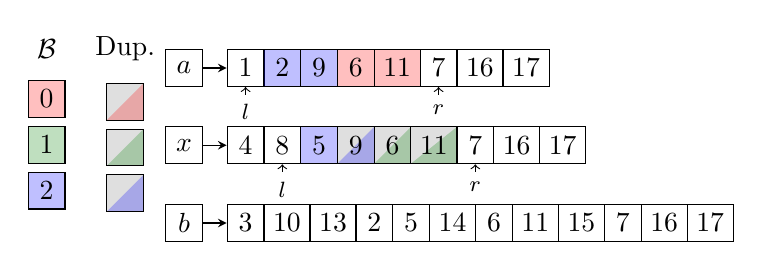
\begin{tikzpicture}
  \newcommand\ptrdown{r}
  \newcommand\ptrup{l}
  \newcommand\ptrupdownlen{0.1}
  \newcommand\listspacing{0.5}
  \newcommand\listpartspacing{0.3}
  \newcommand\arraypartspacing{0.015} % 0.03 for thick
  \newcommand\listdir{right}
  \newcommand\lbldir{below}

  \tikzset{ilentry/.style={draw, minimum width=0.4675cm, minimum height=0.4675cm}}
  \tikzset{processedilentry/.style={ilentry, fill opacity=0.25, text opacity=1}}
  \tikzset{ilentrylb0/.style={processedilentry, fill=red}}
  \tikzset{ilentrylb1/.style={processedilentry, fill=black!50!green}}
  \tikzset{ilentrylb2/.style={processedilentry, fill=blue}}
  \tikzset{ilentrylb3/.style={processedilentry, fill=magenta}}
  %\tikzset{ilentrylb5/.style={processedilentry, fill=gray}}
  \tikzset{ptr/.style={->, >=stealth}}
  \tikzset{
  diagonal fill/.style 2 args={fill=#2, path picture={
    \fill[#1] (path picture bounding box.south west) -|
              (path picture bounding box.north east) -- cycle;}}}
  \tikzset{ilentrylb0seen/.style={processedilentry, diagonal fill={red}{gray}}}
  \tikzset{ilentrylb1seen/.style={processedilentry, diagonal fill={black!50!green}{gray}}}
  \tikzset{ilentrylb2seen/.style={processedilentry, diagonal fill={blue}{gray}}}
  \tikzset{ilentrylb3seen/.style={processedilentry, diagonal fill={magenta}{gray}}}

  % inverted lists
  \node[ilentry] at (0, 0) (il1) {$a$};
  \foreach \label/\labelid [count=\prevlabelid from 1] in {x/2, b/3}{
    \node[ilentry, \lbldir=\listspacing of il\prevlabelid] (il\labelid) {$\label$};
  }

  \node[ilentry, \listdir=\listpartspacing of il1] (il1-1) {$1$};
  \draw[ptr] (il1) -- (il1-1);
  \foreach \poid/\idx/\style [count=\x from 1] in {2/2/ilentrylb2, 9/3/ilentrylb2, 6/4/ilentrylb0, 11/5/ilentrylb0, 7/6/ilentry, 16/7/ilentry, 17/8/ilentry}{
    \node[\style, \listdir=-\arraypartspacing of il1-\x] (il1-\idx) {$\poid$};
  }

  \node[ilentry, \listdir=\listpartspacing of il2] (il2-1) {$4$};
  \draw[ptr] (il2) -- (il2-1);
  \foreach \poid/\idx/\style [count=\x from 1] in {8/2/ilentry, 5/3/ilentrylb2, 9/4/ilentrylb2seen, 6/5/ilentrylb1seen, 11/6/ilentrylb1seen, 7/7/ilentry, 16/8/ilentry, 17/9/ilentry}{
    \node[\style, \listdir=-\arraypartspacing of il2-\x] (il2-\idx) {$\poid$};
  }

  \node[ilentry, \listdir=\listpartspacing of il3] (il3-1) {$3$};
  \draw[ptr] (il3) -- (il3-1);
  \foreach \poid/\idx/\style [count=\x from 1] in {10/2/ilentry, 13/3/ilentry, 2/4/ilentry, 5/5/ilentry, 14/6/ilentry, 6/7/ilentry, 11/8/ilentry, 15/9/ilentry, 7/10/ilentry, 16/11/ilentry, 17/12/ilentry}{
    \node[\style, \listdir=-\arraypartspacing of il3-\x] (il3-\idx) {$\poid$};
  }

  \node[left=3*\listspacing of il1.north] (legend-t) {$\mathcal{B}$};
  \node[ilentrylb0, \lbldir=\listpartspacing/2 of legend-t] (legend-b0) {$0$};
  \foreach \b [count=\bip from 0] in {1, 2}{
    \node[ilentrylb\b, \lbldir=\listpartspacing/3 of legend-b\bip] (legend-b\b) {$\b$};
  }

  \node[right=0.5*\listspacing of legend-t] (legend2-t) {Dup.};
  \node[ilentrylb0seen, \lbldir=\listpartspacing/2 of legend2-t] (legend2-b0) {};
  \foreach \b [count=\bip from 0] in {1, 2}{
    \node[ilentrylb\b seen, \lbldir=\listpartspacing/3 of legend2-b\bip] (legend2-b\b) {};
  }

  % current
  \foreach \listidx/\pup/\pdown in {1/1/6, 2/2/7}{
    \draw[<-] (il\listidx-\pup.south) -- ++(0, -\ptrupdownlen) node[\lbldir] {\footnotesize$\ptrup$};
    \draw[<-] (il\listidx-\pdown.south) -- ++(0, -\ptrupdownlen) node[\lbldir] {\footnotesize$\ptrdown$};
  }
\end{tikzpicture}}

\end{document}
